% Redefinir el título del apéndice
\titleformat{\section}[block]
{\normalfont\Large\bfseries}
{}
{0pt}
{}

\section*{Anexos}
\addcontentsline{toc}{section}{Anexos}

% Reiniciar contadores
\setcounter{figure}{0}
\setcounter{table}{0}

% Redefinir formato de numeración
\renewcommand{\thefigure}{A\arabic{figure}}
\renewcommand{\thetable}{A\arabic{table}}


\begin{table}[H]
    \centering
    \caption{Genomas de referencia de los que se obtuvieron las secuencias de nsp10/14/16.}\label{tab:refgenomes}
    \scriptsize 
    \setlength{\tabcolsep}{12pt}
    \begin{tabularx}{\textwidth}{@{}>{\raggedright\arraybackslash}p{4cm}>{\raggedright\arraybackslash}p{4.5cm}>{\raggedright\arraybackslash}p{3cm}>{\raggedright\arraybackslash}X@{}}
    \toprule
    \textbf{Especie}                                                & \textbf{Nombre común}                                & \textbf{Abreviatura}                          & \textbf{ID GenBank}   \\ \midrule
    \textbf{Género \textit{Alphacoronavirus}}                                                                                                                                                      \\ \midrule
    \textit{Alphacoronavirus AMALF}                                 & bat alphacoronavirus isolate AMALF                   & BtCoV-AMA-L-F                                 &  MT663548             \\
    \textit{Bat coronavirus CDPHE15}                                & bat coronavirus CDPHE15                              & BtCoV CDPHE15                                 &  KF430219             \\
    \textit{Alphacoronavirus CHB25}                                 & Hipposideros pomona bat coronavirus CHB25            & HipPBCoV-CHB25                                &  MN611525             \\
    \textit{Alphacoronavirus WA3607}                                & alphacoronavirus sp. WA3607                          & ACoV-WA3607                                   &  MK472070             \\
    \textit{Bat coronavirus HKU10}                                  & Rousettus bat coronavirus HKU10                      & BtCoV HKU10                                   &  JQ989270             \\
    \textit{Rhinolophus ferrumequinum alphacoronavirus HuB-2013}    & BtRf-AlphaCoV/HuB2013                                & BtRf-AlphaCoV                                 &  KJ473807             \\
    \textit{Human coronavirus 229E}                                 & human coronavirus 229E                               & $HCoV\_{229E}$                                &  AF304460             \\
    \textit{Human coronavirus 229E}                                 & human coronavirus 229E                               & $HCoV\_{229E}$                                &  JX503061             \\
    \textit{Lucheng Rn rat coronavirus}                             & Lucheng Rn rat coronavirus                           & LRNV                                          &  KF294380             \\
    \textit{Mink coronavirus 1}                                     & mink coronavirus                                     & MCoV                                          &  HM245925             \\
    \textit{Miniopterus bat coronavirus 1}                          & Miniopterus bat coronavirus 1                        & $Mi-BatCoV\_{1A}$                             &  EU420138             \\
    \textit{Miniopterus bat coronavirus HKU8}                       & Miniopterus bat coronavirus                          & $HKU8Mi-BatCoV\_{HKU8}$                       &  EU420139             \\
    \textit{Myotis ricketti alphacoronavirus Sax-2011}              & BtMr-AlphaCoV/SAX2011                                & BtMr-AlphaCoV                                 &  KJ473806             \\
    \textit{Alphacoronavirus HKU33}                                 & Tylonycteris bat coronavirus HKU33                   & TyBCoV-HKU33                                  &  MK720944             \\
    \textit{Alphacoronavirus WA2028}                                & alphacoronavirus sp. WA2028                          & ACoV-WA2028                                   &  MK472068             \\
    \textit{Nyctalus velutinus alphacoronavirus SC-2013}            & BtNv-AlphaCoV/SC2013                                 & BtNv-AlphaCoV                                 &  KJ473809             \\
    \textit{Pipistrellus kuhlii coronavirus 3398}                   & alphacoronavirus bat coronavirus                     & PK-BatCoV                                     &  MH938449             \\
    \textit{Alphacoronavirus BT020}                                 & bat alphacoronavirus $BtCoV/020\_{16/M.dau/FIN/2016}$     & $BtCoV/020\_{16/M.dau}$ /FIN/2016        &  MG923574             \\
    \textit{Alphacoronavirus WA1087}                                & alphacoronavirus sp. WA1087                          & ACoV-WA1087                                   &  MK472067             \\
    \textit{Porcine epidemic diarrhea virus}                        & porcine epidemic diarrhea virus                      & PEDV                                          &  AF353511             \\
    \textit{Scotophilus bat coronavirus 512}                        & Scotophilus bat coronavirus 512                      & $Sc-BatCoV\_{512}$                            &  DQ648858             \\
    \textit{Rhinolophus bat coronavirus HKU2}                       & Rhinolophus bat coronavirus HKU2                     & $Rh-BatCoV\_{HKU2}$                           &  EF203064             \\
    \textit{Human coronavirus NL63}                                 & human coronavirus NL63                               & $HCoV\_{NL63}$                                &  AY567487             \\
    \textit{NL63-related bat coronavirus strain BtKYNL63--9b}       & NL63-related bat coronavirus                         & BtKYNL63                                      &  KY073745             \\
    \textit{Sorex araneus coronavirus T14}                          & common shrew coronavirus Tibet-2014                  & $Sa-CoV\_{T14}$                               &  KY370053             \\ 
    \textit{Suncus murinus coronavirus X74}                         & Suncus murinus coronavirus Xingguo-74                & $Sm-CoV\_{X74}$                               &  KY967715             \\
    \textit{Alphacoronavirus 1}                                     & transmissible gastroenteritis virus                  & TGEV                                          &  AJ271965             \\ 
    \end{tabularx}
\end{table}

\begin{table}[H]
    \centering
    \scriptsize 
    \setlength{\tabcolsep}{12pt}
    \begin{tabularx}{\textwidth}{@{}>{\raggedright\arraybackslash}p{4cm}>{\raggedright\arraybackslash}p{4.5cm}>{\raggedright\arraybackslash}p{3cm}>{\raggedright\arraybackslash}X@{}}
    \midrule
    \textbf{Género \textit{Betacoronavirus}}                                                                                                                                                       \\ \midrule
    \textit{Betacoronavirus 1}                                      & human coronavirus OC43                               & $HCoV\_{OC43}$                                &  AY585228             \\
    \textit{China Rattus coronavirus HKU24}                         & betacoronavirus HKU24                                & $ChRCoV\_{HKU24}$                             &  KM349742             \\
    \textit{Human coronavirus HKU1}                                 & human coronavirus HKU1                               & $HCoV\_{HKU1}$                                &  AY597011             \\
    \textit{Murine coronavirus}                                     & murine hepatitis virus                               & MHV                                           &  AY700211             \\
    \textit{Myodes coronavirus 2JL14}                               & Myodes rufocanus vole coronavirus 2/JL2014           & $MrufCoV\_{2JL14}$                            &  KY370046             \\    
    \textit{Murine coronavirus}                                     & murine hepatitis virus                               & MHV                                           &  AY700211             \\
    \textit{Myodes coronavirus 2JL14}                               & Myodes rufocanus vole coronavirus 2/JL2014           & $MrufCoV\_{2JL14}$                            &  KY370046             \\ 
    \textit{Bat Hp-betacoronavirus}                                 & bat Hp-betacoronavirus/Zhejiang2013                  & $Bat\_{Hp-BetaCoV}$                           &  KF636752             \\    
    \textit{Hedgehog coronavirus 1}                                 & hedgehog coronavirus 1                               & EriCoV                                        &  KC545383             \\
    \textit{Middle East respiratory syndrome-related coronavirus}   & Middle East respiratory syndrome-related coronavirus & MERS-CoV                                      &  JX869059             \\
    \textit{Pipistrellus bat coronavirus HKU5}                      & Pipistrellus bat coronavirus HKU5                    & $Pi-BatCoV\_{HKU5}$                           &  EF065509             \\
    \textit{Tylonycteris bat coronavirus HKU4}                      & Tylonycteris bat coronavirus HKU4                    & $Ty-BatCoV\_{HKU4}$                           &  EF065505             \\
    \textit{Eidolon bat coronavirus C704}                           & Eidolon helvum bat coronavirus CMR704-P12            & $Ei-BatCoV\_{C704}$                           &  MG693168             \\
    \textit{Rousettus bat coronavirus GCCDC1}                       & Rousettus bat coronavirus                            & $Ro-BatCoV\_{GCCDC1}$                         &  KU762338             \\
    \textit{Rousettus bat coronavirus HKU9}                         & Rousettus bat coronavirus HKU9                       & $Ro-BatCoV\_{HKU9}$                           &  EF065513             \\
    \textit{Severe acute respiratory syndrome-related coronavirus}  & severe acute respiratory syndrome coronavirus        & SARS-CoV                                      &  AY274119             \\
    \textit{Severe acute respiratory syndrome-related coronavirus}  & severe acute respiratory syndrome-related coronavirus & SARSr-CoV                                    &  KY352407             \\
    \textit{Severe acute respiratory syndrome-related coronavirus}  & severe acute respiratory syndrome coronavirus 2      & SARS-CoV-2                                    &  MN908947             \\ \midrule
    \textbf{Género \textit{Deltacoronavirus}}                                                                                                                                                      \\ \midrule
    \textit{Wigeon coronavirus HKU20}                               & wigeon coronavirus HKU20                             & $WiCoV\_{HKU20}$                              &  JQ065048             \\
    \textit{Bulbul coronavirus HKU11}                               & bulbul coronavirus HKU11                             & $BulCV\_{HKU11}$                              &  FJ376619             \\
    \textit{Common moorhen coronavirus HKU21}                       & common moorhen coronavirus HKU21                     & $CMCoV\_{HKU21}$                              &  JQ065049             \\
    \textit{Coronavirus HKU15}                                      & porcine coronavirus HKU15                            & $PoCoV\_{HKU15}$                              &  JQ065043             \\
    \textit{Munia coronavirus HKU13}                                & munia coronavirus HKU13                              & $MunCV\_{HKU13}$                              &  FJ376622             \\
    \textit{White-eye coronavirus HKU16}                            & white-eye coronavirus HKU16                          & $WECoV\_{HKU16}$                              &  JQ065044             \\
    \textit{Night heron coronavirus HKU19}                          & night heron coronavirus HKU19                        & $NHCoV\_{HKU19}$                              &  JQ065047             \\ \midrule
    \textbf{Género \textit{Gammacoronavirus}}                                                                                                                                                      \\ \midrule
    \textit{Goose coronavirus CB17}                                 & Canada goose-Branta canadensis-coronavirus-Cambridge Bay 2017 & $BcanCoV\_{CB17}$                    &  MK359255             \\ 
    \textit{Beluga whale coronavirus SW1}                           & beluga whale coronavirus                             & BWCoV                                         &  EU111742             \\
    \end{tabularx}
\end{table}

\begin{table}[H]
    \centering
    \scriptsize 
    \setlength{\tabcolsep}{12pt}
    \begin{tabularx}{\textwidth}{@{}>{\raggedright\arraybackslash}p{4cm}>{\raggedright\arraybackslash}p{4cm}>{\raggedright\arraybackslash}p{3cm}>{\raggedright\arraybackslash}X@{}}
    \textit{Avian coronavirus}                                      & infectious bronchitis virus                          & IBV                                            &  M95169              \\
    \textit{Avian coronavirus 9203}                                 & infectious bronchitis virus Ind-TN92--03             & $ACoV\_{9203}$                                 &  KR902510            \\
    \textit{Duck coronavirus 2714}                                  & duck coronavirus DK/GD/27/2014                       & $DuCoV\_{2714}$                                &  KM454473            \\ \bottomrule
    \end{tabularx}
\end{table}

\begin{table}[H]
    \centering
    \caption{Combinación de colores de Clustal, tomada de la web de Jalview 
    (\cite{noauthor_clustal_nodate}). A cada residuo en el alineamiento se le 
    asigna un color según los criterios siguientes.}
    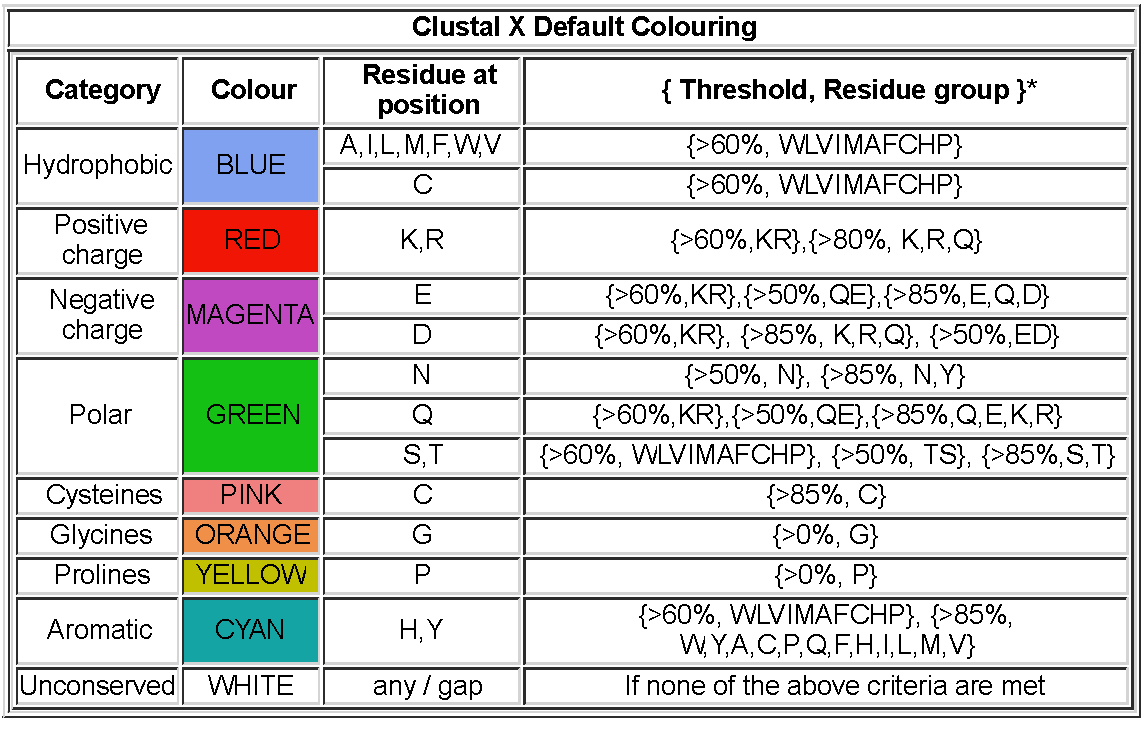
\includegraphics[width=\textwidth]{img/tabA2.pdf}
    \vspace{0.5cm}
    \begin{minipage}{\textwidth}
        \footnotesize
        *Los criterios de coloración se indican de la forma condicional 
        \{\textgreater{X\%}, y, z\}, siendo coloreadas aquellas posiciones del alineamiento
        con la representación porcentual mínima (X) de determinados aminoácidos 
        combinables (y, z). De este modo, una posición con K o R se coloreará de
        rojo si la columna contiene más de un 60\% de residuos K y/o R, o más de
        un 80\% de residuos K, R y Q.
    \end{minipage}
\end{table}
